\documentclass[11pt]{article}

\usepackage{latexsym}
\usepackage{amsmath}
\usepackage{amssymb}
\usepackage{amsthm}
\usepackage{graphicx}
\usepackage{wrapfig}
\usepackage{pseudocode}
\usepackage{url}
\usepackage{array}
\usepackage{amsmath}
\usepackage{algorithm}
\usepackage[noend]{algpseudocode}
\usepackage{makebox}
\usepackage{mathtools}
\usepackage{svg}
\usepackage{xcolor}
\usepackage{subfig}
\usepackage{multirow}
\usepackage{color}
\usepackage{float}
\usepackage{caption}
\usepackage[backref, colorlinks=true, citecolor=red, urlcolor=blue, pdfauthor={Jyh-Ming Lien}]{hyperref}


\newcommand{\handout}[5]{
  \noindent
  \begin{center}
  \framebox{
    \vbox{
      \hbox to 5.78in { {\bf } \hfill #2 }
      \vspace{4mm}
      \hbox to 5.78in { {\Large \hfill #5  \hfill} }
      \vspace{2mm}
      \hbox to 5.78in { {\em #3 \hfill #4} }
    }
  }
  \end{center}
  \vspace*{4mm}
}

\newcommand{\lecture}[4]{\handout{#1}{#2}{#3}{#4}{#1}}

\newtheorem{theorem}{Theorem}
\newtheorem{corollary}[theorem]{Corollary}
\newtheorem{lemma}[theorem]{Lemma}
\newtheorem{observation}[theorem]{Observation}
\newtheorem{proposition}[theorem]{Proposition}
\newtheorem{definition}[theorem]{Definition}
\newtheorem{claim}[theorem]{Claim}
\newtheorem{fact}[theorem]{Fact}
\newtheorem{assumption}[theorem]{Assumption}

% 1-inch margins, from fullpage.sty by H.Partl, Version 2, Dec. 15, 1988.
\topmargin 0pt
\advance \topmargin by -\headheight
\advance \topmargin by -\headsep
\textheight 8.9in
\oddsidemargin 0pt
\evensidemargin \oddsidemargin
\marginparwidth 0.5in
\textwidth 6.5in

\parindent 0in
\parskip 1.5ex
%\renewcommand{\baselinestretch}{1.25}

\begin{document}

\lecture{Midterm Exam Report}{Fall 2015}{Yunjoo Park}{Advance Algorithm Programming}

\section{Summary of the two methods}
A \textit{Voronoi diagram} of a given point set $P$ is the subdivision of the plane into $n$ cells based on distance to points, one for each site of $P$, with the property that a point $q$ lies in the cell corresponding to a site $p_i$ if and only if $dist(q, p_i ) < dist(q, p_j )$ for each $p_j \in P$ with $j \ne i$\cite{computational-geometry-book}. A \textit{Centroidal Voronoi Tessellation} (CVT) is a special type of Voronoi diagrams. In the CVT, the point of each voronoi cell is the center of mass. Especially, a \textit{Weighted Centroidal Voronoi Diagram} (WCVT) is a CVT in which each centroid is weighted according to a certain function. 
There are two methods to generate stipple drawings from images using weighted centroidal Voronoi diagrams. Both are based on the paper, "Weighted Voronoi Stipples"\cite{weighted-voronoi-stipples}. One is implemented by hedcuter. The other is implemted by voronoi method. Both generate well-spaced sets of points.
\subsection{hedcuter method}
This method is one way to generate stipple drawings from input image. This uses weighted centroidal voronoi diagram. Input is any image file and output is svg file. The program could have options below.
\begin{table}[hbt]
\centering
\begin{tabular}{|l||l|l|l|}  
\hline
Parameter & Arg. & default & Description\\
\hline\hline
-debug & X & false & Output with debugging information\\  
\hline
-n & O & 1000 & Sample size\\
\hline
-uniform\_radius & X & false & True, then all disks have the same radius\\
\hline
-radius & O & 1 &
\vtop{\hbox{\strut  If uniform\_disk is true, all disks have the disk size of the value.}\hbox{\strut Otherwise, the largest disks will have the disk size of the value.}} \\
\hline
-iteration & O & 100 & Centroidal voronoid tessellation iteration limit\\
\hline
-maxD & O & 1.01f & Max of site displacement\\
\hline
-black & X & false & True, then black disk\\
\hline
\end{tabular}
\caption{Hedcuter method's options}
\label{hedcutermethodoptions}
\end{table}

This program uses Discrete Stippling algorithm\cite{weighted-voronoi-stippling} to stipple an image quickly.

\begin{figure}[hbt]
\centering
\begin{minipage}{0.7\textwidth}

\begin{algorithm}[H]
\caption{Discrete Stippling}
\label{discretestippling}
\begin{algorithmic}
\ForAll{pixel positions $(x, y) \in [0,1]$ x $[0,1]$} 

	\State Map image value at $(x, y)$ to stipple level $l$
	\State Copy stipples on level $l$ inside $(x-\frac{1}{2}, y-\frac{1}{2})$ x $(x+\frac{1}{2}, y+\frac{1}{2})$
\EndFor
\end{algorithmic}
\end{algorithm}
\end{minipage}
\end{figure}

\clearpage
In the program, build process undergoes several steps. 
\begin{description}
  \item[First] Initialize sample points
  \item[Second] Compute a Weighted Voronoi Tessellation
	\begin{enumerate}
	  \item compute voronoi
	  \item move the site to the center of its coverage
	\end{enumerate}
  \item[Third] Create disks
\end{description}
The method use 256 as the number required in a pure black image. We call the number $N$.
\\ \\
First of all, hedcuter generates sample initial $n$ points. To be specific, $n$ is initialized by \textit{user}, or default value is 1000. For generating random points, it uses RNG (Random Number Generator). The random points are generated and distributed uniformly. The hedcuter calculates their value based on each color. If the point is close to black, the value is close to 0. On the contrary, if the point is close to white, the value is close to 1. This value is used to determines which points are appropriate. The points are decided whether to keep or not by comparing the value with a random number sampled from the gaussian distribution. Thus, the black has higher probability.
\\ \\
Second part is main of the hedcuter. At first, the hedcuter copies all points to \textit{site of cells} and calculate \textit{distance} for cells. The distance of each cell is obtained by converting its color intensity to distance value [0, 1] by equation (\ref{eq:colortodist}). Let $indensity(c)$ be the color intensity and $distance(c)$ be the distance of the stipple.

\begin{equation}
distance(c) = \frac{\left(N-intensity\left(c\right)\right)*1.0f}{N}
\label{eq:colortodist}
\end{equation}

And then, sort cells using heap. The next step is about propagation. For each cell, the hedcuter calculate new distance of its neighbors. Neighbors are the points which are 3X3 matrix around the stipple.

\begin{equation}
distance_{new}(neighbor) = distance(c) + distance(neighbor)
\label{eq:distance}
\end{equation}

If the calculated distance is less than the distance of the neighbor, push the neighbor to heap with the new distance. Finally, after the propagation step, the hedcuter collects cells by pushing points to ceverage of corresponding cell and removes empty cells. For the collected cells, the hedcuter computes weighted average distance of each cell and updates the site of the cell to the new position using the distance. Repeat these process while satisfying the following conditions.
\begin{itemize}
  \item the max of the displacement of site at each iteration  $<$ max\_site\_displacement (1.01f)
  \item the number of iterations $<$ iteration\_limit (option: -iteration)
\end{itemize}

\subsection{voronoi method}
This method is also one way to generate stipple drawings from input image. This uses weighted centroidal voronoi diagram. Input file must be a PNG image. The program could have options below. Specifically, input and output are required\cite{saliences}.
\begin{table}[hbt]
\centering
\begin{tabular}{|l||l|l|l|}  
\hline
Param. & Arg. & default & Description\\
\hline\hline
-I & O &  & Must be a PNG file.\\  
\hline
-O & O &  & The name of the file to output\\
\hline
-s & O & 4000 & The number of stipple points to render.\\
\hline
-c & X & OFF & Off, output in black and white\\
\hline
-t & O & 0.1 & The cut-off point for the convergence of the stippled output.\\
\hline
-n & X & OFF & Stipple points will not overlap.\\
\hline
-f & X & OFF & ON, then all stipple points have the equal size of radius.\\
\hline
-z & O & 1.0 & The radius of each stipple is multiplied by this value.\\
\hline
-p & O & 5 & Controls the tile size of centroid computations.\\
\hline
-l & X & OFF & ON, then produce an output log.\\
\hline
\end{tabular}
\caption{Voronoi method's options}
\label{voronoimethodoptions}
\end{table}
\\
As I mentioned before, in CVT, each generating point lies exactly on the centroid of its voronoi region. The centroid of a region is defined as 
\begin{equation}
C_i = \frac{\int_{A} x\rho(x), dA}{\int_{A} \rho(x), dA}
\label{eq:centroid}
\end{equation}
where $A$ is the region of the cell, $x$ is the position and $\rho(x)$ is the density function. A centroidal voronoi diagram is a minimum-energy configuration in the sense that it minimize $\int_{A}\rho(x){|C_i-x|}^2$.\cite{weighted-voronoi-stipples}
This program uses Lloyd's algorithm\cite{weighted-voronoi-stippling} to generate a centroidal Voronoi diagram from any set of generating points.
\begin{figure}[hbt]
\centering
\begin{minipage}{0.7\textwidth}

\begin{algorithm}[H]
\caption{Lloyd's method}
\label{lloydmethod}
\begin{algorithmic}
\While{generating points $x_i$} 
	\State Compute the Voronoi diagram of $x_i$
	\State Compute the centroids $C_i$ using equation (\ref{eq:centroid})
	\State Move each generating point $x_i$ to its centroid $C_i$
\EndWhile
\end{algorithmic}
\end{algorithm}
\end{minipage}
\end{figure}
\\
The algorithm find evenly spaced sets of points in subsets of Euclidean spaces, and partitions of these subsets into well-shaped and uniformly sized convex cells. That is, Under the algorithm, a voronoi diagram become a centroidal voronoi diagram through relaxation step.
\clearpage
The program consists of the following several steps.
\begin{description}
  \item[First] Create stippler
  \item[Second] Loop while (average displacement $>$ threshold)
	\begin{enumerate}
	  \item distribute stipples
		\begin{enumerate}
	     \item create voronoi diagram	
	     \item redistribute stipples
		\end{enumerate}
	\end{enumerate}
  \item[Third] Render
\end{description}

In the first step, creates initial stipples. The second step is the main part. Firstly, in the \textit{createVoronoiDiagram()} part, generates a voronoi diagram using stipples. Second, in the \textit{redistributeStipples()} part, calcuates the centroid of a cell using edges of the cell. To be specific, in the process of calcuating the centroid, creates and computes clip lines. Each clip line is extension of each edge. Thus, the clip lines form a polygon. Tests whether each point around the stipple is outside of the polygon or not. gets the density from image for inside points, calculates the density of the cell, and returns the center and radius of the cell. Updates stipples of voronoi diagram with the centroid. After updating, calculates the average displacement of stipples, denoted by $t$. Repeat this second step while $t$ is greater than the \textit{threshold}.

\section{Comparison of the two methods}
\subsection{Do you get the same results by running the same program on the same image multiple times?}%2.1
\begin{enumerate}
	\item Hedcuter
	\begin{figure}[htbp]
	  \centering
	  
\includegraphics[width=.23\textwidth]{FIGS/hedcut/svg/phoenix-5000-h1}
	  
\includegraphics[width=.23\textwidth]{FIGS/hedcut/svg/phoenix-5000-h2}
	  
\includegraphics[width=.23\textwidth]{FIGS/hedcut/svg/phoenix-5000-h3}
	  \caption{phoenix with 5000}
	  \label{fig:hedcuterphoenix}
	\end{figure}

	\item Voronoi
	\begin{figure}[htbp]
 	 \centering
 	 
\includegraphics[width=.23\textwidth]{FIGS/voronoi/svg/phoenix-5000-v1}
 	 \includegraphics[width=.23\textwidth]{FIGS/voronoi/svg/phoenix-5000-v2}
 	 \includegraphics[width=.23\textwidth]{FIGS/voronoi/svg/phoenix-5000-v3}
 	 \caption{phoenix with 5000}
	\end{figure}
\end{enumerate}
While I got the different outputs by running the hedcuter program on the same image multiple times, I obtained the same outputs by running the voronoi program. The hedcuter generates initial points randomly and make a CVT under limit iteration and given max site displacement. Since initial points set are different, the results of propagation are also changed. On the other hand, the voronoi program has the same initial points and repeats the series of process until the average of displacement of points is small enough. Thus, I could get the same output multiple times.

\subsection{If you vary the number of the disks in the output images, do these implementations produce the same distribution in the final image? If not, why?}%2.2
Figure \ref{fig:varydiskhedcut} and Figure \ref{fig:varydiskvoronoi} show the output image of klaymen of Hedcuter and Voronoi. Both methods produce the different distribution in the final image when the the number of the disks varies. As the number of the disks increases, they generate the more detailed results.

	\begin{figure}[ht] 
	\begin{center} 
	\subfloat[2981 disks]{
		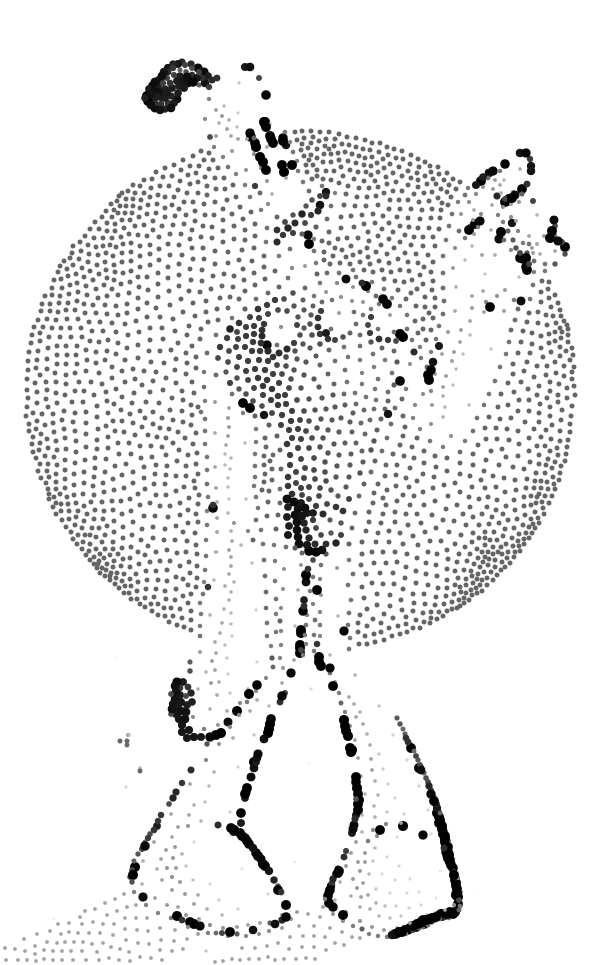
\includegraphics[width=0.18\textwidth]{FIGS/hedcut/svg/klaymen-3000-h}}
		\hspace{5mm}
	\subfloat[4943 disks]{
		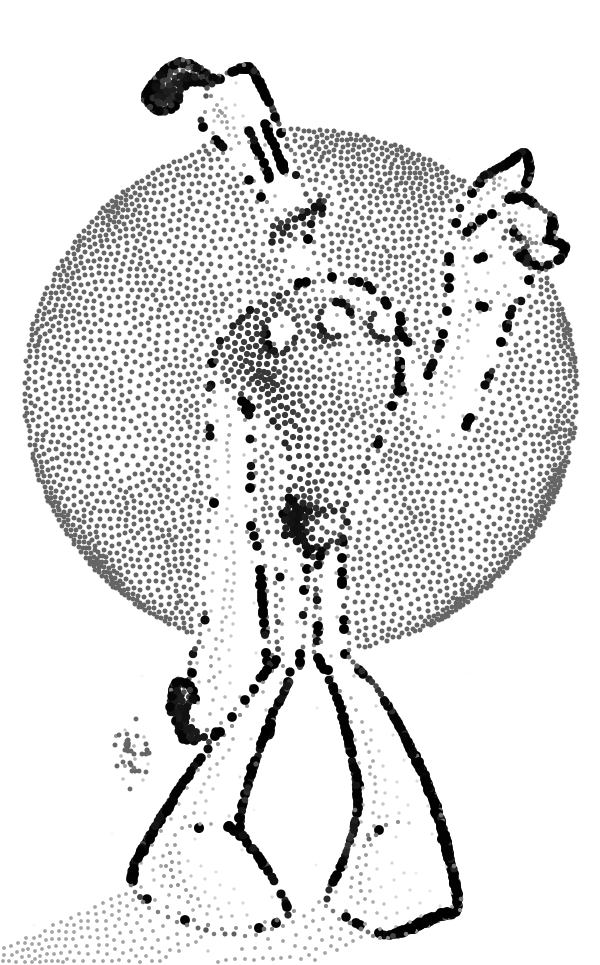
\includegraphics[width=0.18\textwidth]{FIGS/hedcut/svg/klaymen-5000-h}}
	\hspace{5mm}
	\subfloat[9829 disks]{
		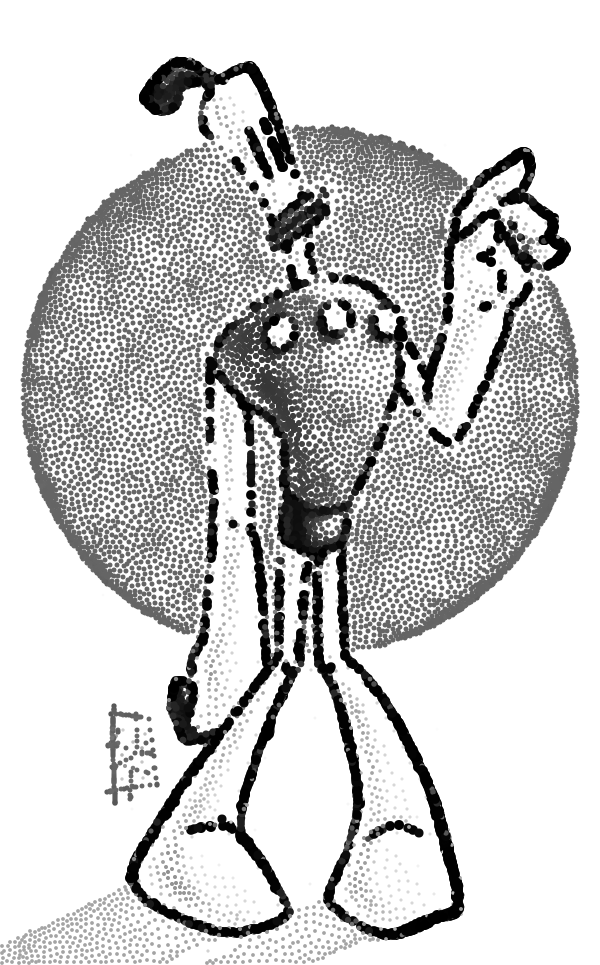
\includegraphics[width=0.18\textwidth]{FIGS/hedcut/svg/klaymen-10000-h}}
	\hspace{5mm}
	\subfloat[55070 disks nonblack]{
		\includegraphics[width=0.18\textwidth]{FIGS/hedcut/svg/klaymen-100000-h-nonblack}}
	\caption{Hedcuter klaymen}
	\label{fig:varydiskhedcut} 
	\end{center} 
	\end{figure}
	\begin{figure}[ht] 
	\begin{center} 
	\subfloat[1000 stipples]{
		
\includegraphics[width=0.18\textwidth]{FIGS/voronoi/svg/klaymen-1000-v}}
		\hspace{5mm}
	\subfloat[5000 stipples]{
		
\includegraphics[width=0.18\textwidth]{FIGS/voronoi/svg/klaymen-5000-v}}
		\hspace{5mm}
	\subfloat[20000 stipples]{
		
\includegraphics[width=0.18\textwidth]{FIGS/voronoi/svg/klaymen-20000-v}}
		\hspace{5mm}
	\subfloat[100000 stipples]{
		\includegraphics[width=0.18\textwidth]{FIGS/voronoi/svg/klaymen-100000-v}}
	\caption{Voronoi klaymen} 
	\label{fig:varydiskvoronoi}
	\end{center} 
	\end{figure}
\clearpage

\subsection{If you vary the number of the disks in the output images, is a method faster than the other?}%2.3
I could not assure that one method is faster than the other. In the hedcuter method, there are some points which oscillate after a few iteration in some cases. Thus, if there is no iteration limit, it will take infinite time because some points will oscillate infinitely. In the voronoi method, the more I increase the number of points, it takes the small number of iteration. Figure \ref{fig:klaymenrunningtimevoronoi} and Figure \ref{fig:einsteinrunningtimevoronoi} show elapsed time of the voronoi as the number of stipples is varied. As the number of points increases, the method becomes faster. However, the elapsed time increases again when the number of points goes beyond a certain level. This is because it takes too much time for each iteration even though there are few iteration.

\begin{figure}[hbpt] 
	\begin{center} 
	\subfloat[1000 stipples]{
		
\includegraphics[width=0.4\textwidth]{FIGS/voronoi/running_time/klaymen-1000-v}}
		\hspace{5mm}
	\subfloat[5000 stipples]{
		
\includegraphics[width=0.4\textwidth]{FIGS/voronoi/running_time/klaymen-5000-v}}

	\subfloat[20000 stipples]{
		\includegraphics[width=0.4\textwidth]{FIGS/voronoi/running_time/klaymen-20000-v2}}
		\hspace{5mm}
	\subfloat[100000 stipples]{
		\includegraphics[width=0.4\textwidth]{FIGS/voronoi/running_time/klaymen-100000-v2}}
	\caption{Elapsed time of Klaymen of Voronoi as a function of the number of stipples} 
	\label{fig:klaymenrunningtimevoronoi}
	\end{center} 
\end{figure}

\begin{figure}[hbpt] 
	\begin{center} 
	\subfloat[100 stipples]{
		\includegraphics[width=0.4\textwidth]{FIGS/voronoi/running_time/einstein-100-v2}}
		\hspace{5mm}
	\subfloat[5000 stipples]{
		\includegraphics[width=0.4\textwidth]{FIGS/voronoi/running_time/einstein-5000-v2}}

	\subfloat[250000 stipples]{
		\includegraphics[width=0.4\textwidth]{FIGS/voronoi/running_time/einstein-250000-v2}}
		\hspace{5mm}
	\subfloat[10000000 stipples]{
		\includegraphics[width=0.4\textwidth]{FIGS/voronoi/running_time/einstein-10000000-v2}}
	\caption{Elapsed time of Klaymen of Voronoi as a function of the number of stipples} 
	\label{fig:einsteinrunningtimevoronoi}
	\end{center} 
\end{figure}


\subsection{Does the size (number of pixels), image brightness or contrast of image increase or decrease their difference?}%2.4
The Hedcuter method uses \textit{-radius} option. When the \textit{-uniform\_radius} option is off, the largest disks will have the disk size of the radius value. On the other hand, the Voronoi method can render without radius limit. As shown in Figure \ref{fig:einsteinmedium100hedcuter} and Figure \ref{fig:einsteinmedium100voronoi}, when the given number of the initial points is small, this option affect the results significantly.  Thus, the number of given points should be large enough to confirm difference.

	\begin{figure}[ht] 
	\begin{center} 
	\subfloat[-radius 5]{
		
\includegraphics[width=0.15\textwidth]{FIGS/hedcut/svg/einstein-medium-100-h-nonblack}}
		\hspace{5mm}
	\subfloat[-radius 10]{
		
\includegraphics[width=0.15\textwidth]{FIGS/hedcut/svg/einstein-medium-100-h-radius10}}
		\hspace{5mm}
	\subfloat[-radius 30]{
		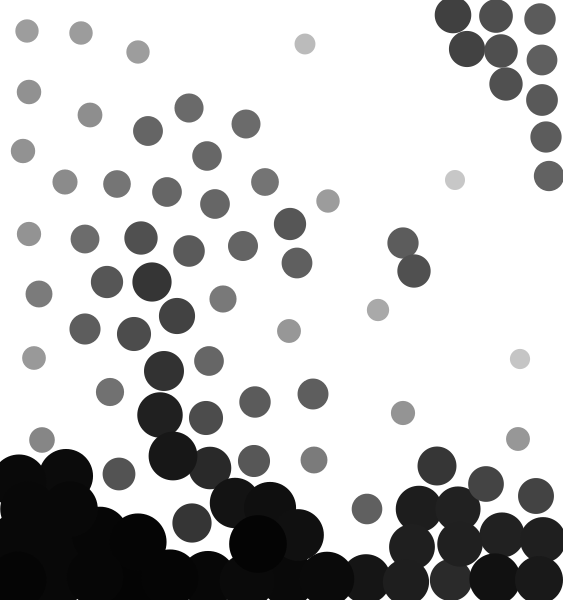
\includegraphics[width=0.15\textwidth]{FIGS/hedcut/svg/einstein-medium-100-h-radius30}}
	\caption{Einstein-medium with 100 sample points of Hedcuter}
	\label{fig:einsteinmedium100hedcuter} 
	\end{center} 
\vspace{-2.0em}
	\end{figure}
	\begin{figure}[ht] 
	\begin{center} 
	\subfloat[-f option]{
		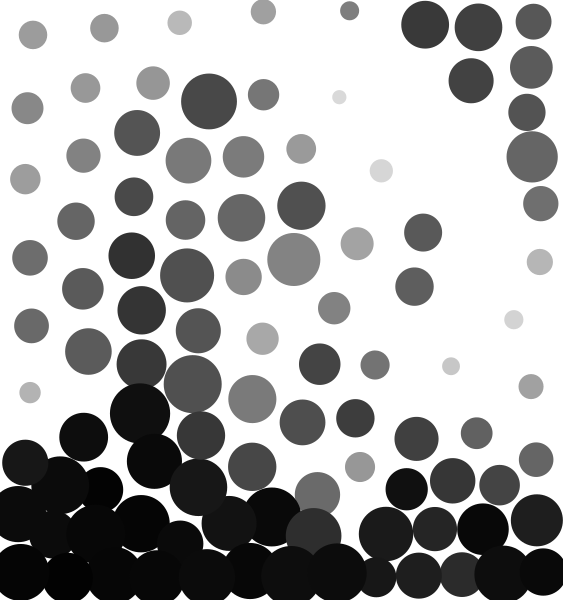
\includegraphics[width=0.15\textwidth]{FIGS/voronoi/svg/einstein-medium-100-v-c}}
		\hspace{5mm}
	\subfloat[no option]{
		
\includegraphics[width=0.15\textwidth]{FIGS/voronoi/svg/einstein-medium-100-v-f}}
	\caption{Einstein-medium with 100 stipples of Voronoi}
	\label{fig:einsteinmedium100voronoi} 
	\end{center} 
	\end{figure}
The resolution of Einstein-medium is 563X600 and the resolution of Einstein-Large 1180X1258. Figure \ref{fig:einsteinmedium5000} shows the result of Einstein-medium with 5000 points. Figure \ref{fig:einstein5000} shows the result of Einstein-Large with 5000 points. The more the number of pixels, the difference increases.
	\begin{figure*}[ht] 
	\begin{center}
\parbox[][][c]{0.48\textwidth }{
	\subfloat[Hedcuter]{
		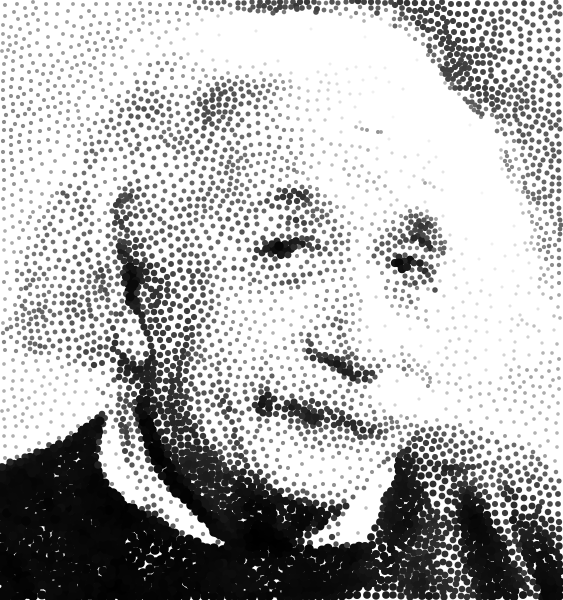
\includegraphics[width=0.23\textwidth]{FIGS/hedcut/svg/einstein-medium-5000-h-nonblack}}
	\subfloat[Voronoi]{
		\includegraphics[width=0.23\textwidth]{FIGS/voronoi/svg/einstein-medium-5000-v-c}}
	\captionof{figure}{Einstein-medium}
	\label{fig:einsteinmedium5000}
}
\parbox[][][c]{0.48\textwidth }{
	\subfloat[Hedcuter]{
		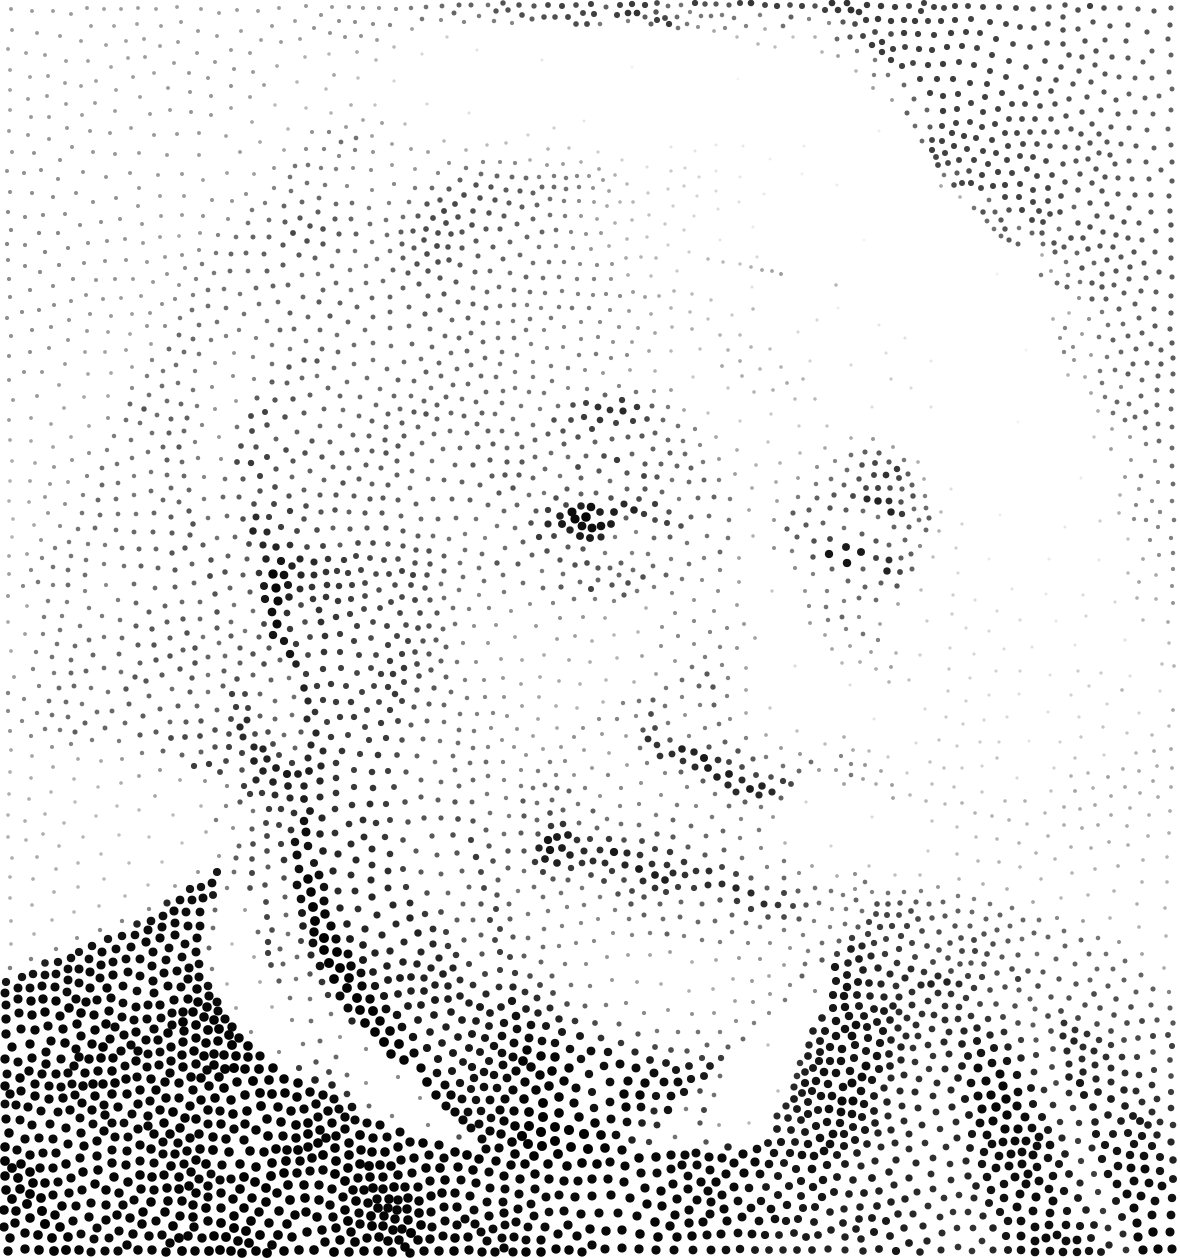
\includegraphics[width=0.23\textwidth]{FIGS/hedcut/svg/einstein-5000-h-nonblack}}
	\subfloat[Voronoi]{
		\includegraphics[width=0.23\textwidth]{FIGS/voronoi/svg/einstein-5000-v-c}}
	\captionof{figure}{Einstein-large}
	\label{fig:einstein5000}
}
	\end{center} 
	\end{figure*}
\clearpage

Also, Figure \ref{fig:einsteinmedium250000} and Figure \ref{fig:einstein250000} shows the results with 250000 points. As shown in the figures, the voronoi method generates the results similart to the input image. This is because the hedcuter method has the iteration limit so that it could not generate the large number of disks; I ran the hedcuter with 500 iteration. Finally, as we can see the figures of Voronoi, it produces similar outputs if the given number of stipples is the same. On the other hand, in the hedcuter method, the quality is degraded in the high resolution under the same number of initial points.
	\begin{figure*}[ht] 
	\begin{center}
\parbox[][][c]{0.48\textwidth }{
	\subfloat[Hedcuter]{
		\includegraphics[width=0.23\textwidth]{FIGS/hedcut/svg/einstein-medium-250000-h-nonblack}}
	\subfloat[Voronoi]{
		\includegraphics[width=0.23\textwidth]{FIGS/voronoi/svg/einstein-medium-250000-v-c}}
	\captionof{figure}{Einstein-medium}
	\label{fig:einsteinmedium250000}
}
\parbox[][][c]{0.48\textwidth }{
	\subfloat[Hedcuter]{
		\includegraphics[width=0.23\textwidth]{FIGS/hedcut/svg/einstein-250000-h-nonblack}}
	\subfloat[Voronoi]{
		\includegraphics[width=0.23\textwidth]{FIGS/voronoi/svg/einstein-250000-v-c}}
	\captionof{figure}{Einstein-large}
	\label{fig:einstein250000}
}
	\end{center} 
	\end{figure*}

Figure \ref{fig:poohgrayscalebhedcut} and Figure \ref{fig:poohgrayscalebhedcut} shows the results as a function of the brightness with 5000 initial points. As we can see, the hedcuter method generates better results under too bright conditions. 
	\begin{figure}[htbp]
	  \centering
	  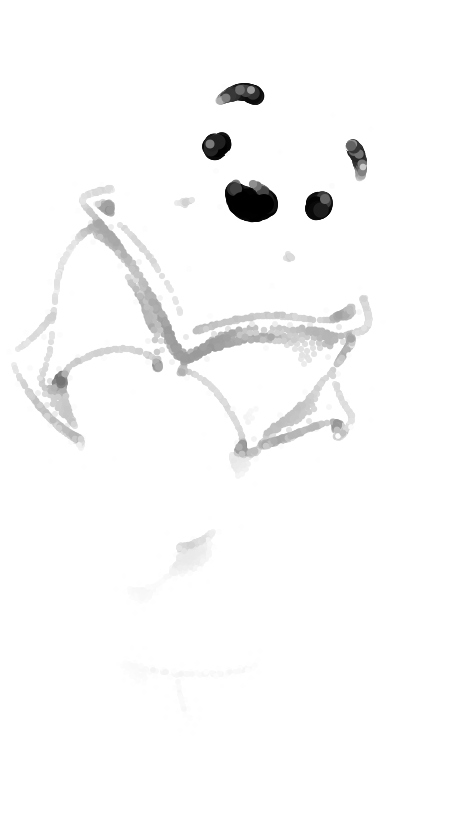
\includegraphics[width=.13\textwidth]{FIGS/pooh_grayscale/b1-h}
	\hspace{3mm}
	  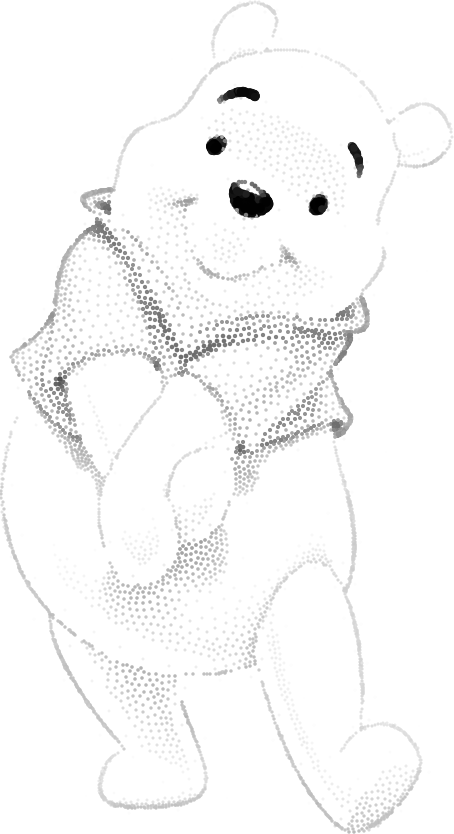
\includegraphics[width=.13\textwidth]{FIGS/pooh_grayscale/b2-h}
	\hspace{3mm}
	  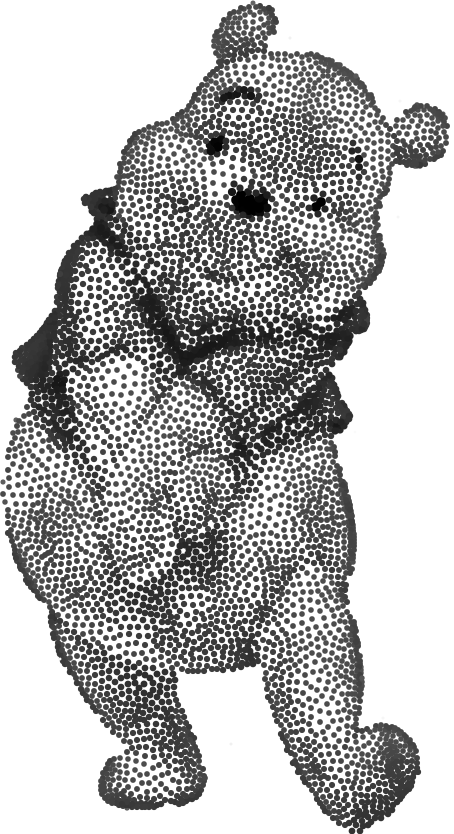
\includegraphics[width=.13\textwidth]{FIGS/pooh_grayscale/b3-h}
	\hspace{3mm}
	  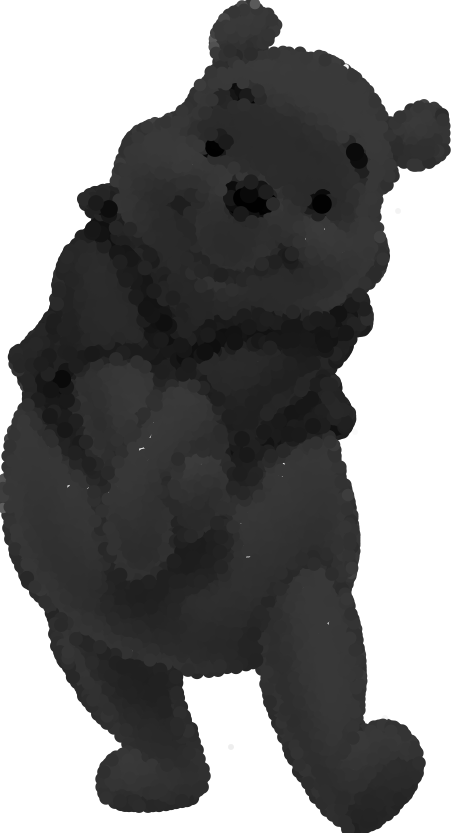
\includegraphics[width=.13\textwidth]{FIGS/pooh_grayscale/b4-h}
	  \caption{pooh of Hedcuter as the brightness changes}
	  \label{fig:poohgrayscalebhedcut}
	\end{figure}
	\begin{figure}[htbp]
	  \centering
	  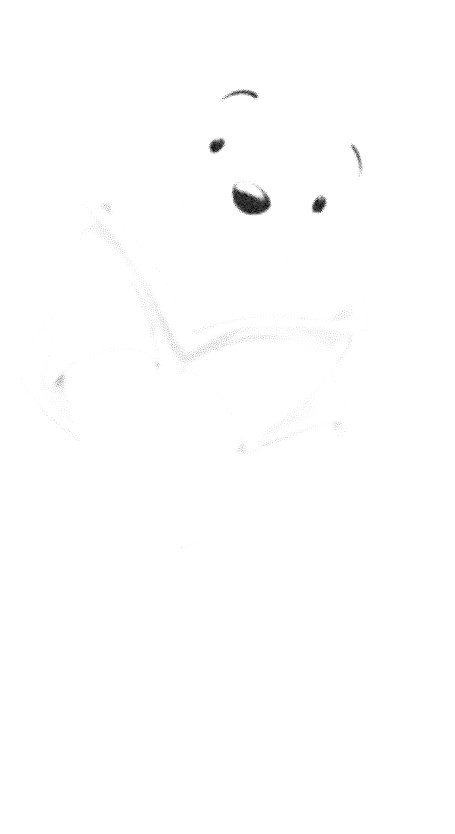
\includegraphics[width=.13\textwidth]{FIGS/pooh_grayscale/b1-v}
	\hspace{3mm}
	  \includegraphics[width=.13\textwidth]{FIGS/pooh_grayscale/b2-v}
	\hspace{3mm}
	  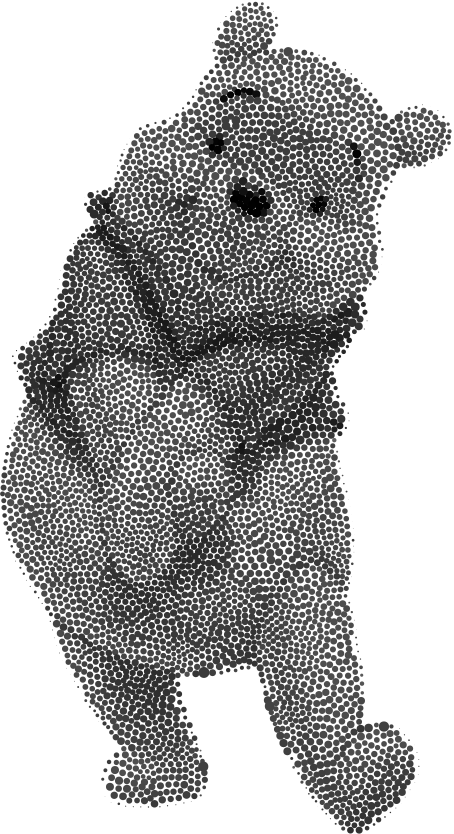
\includegraphics[width=.13\textwidth]{FIGS/pooh_grayscale/b3-v}
	\hspace{3mm}
	  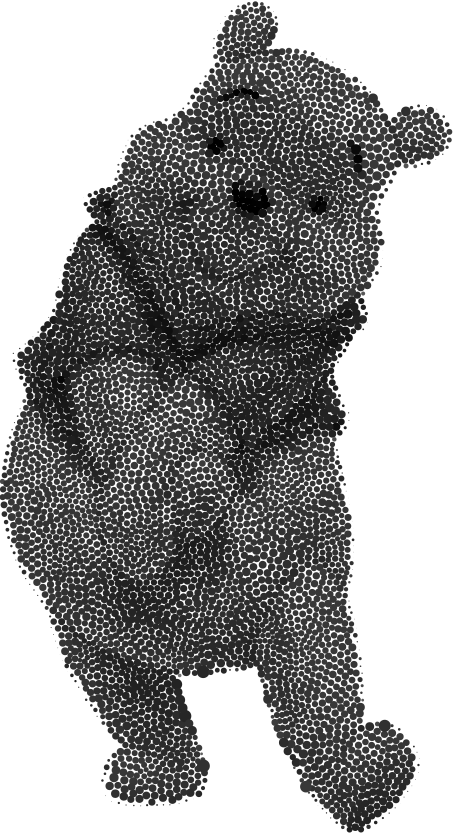
\includegraphics[width=.13\textwidth]{FIGS/pooh_grayscale/b4-v}
	  \caption{pooh of Voronoi as the brightness changes}
	  \label{fig:poohgrayscalebhedcut}
	\end{figure}

Figure \ref{fig:poohgrayscalechedcut} and Figure \ref{fig:poohgrayscalecvoronoi} shows the results as a function of the contrast with 5000 initial points. In bright conditions, the hedcuter produces a better result. Similarly, the hedcuter method seem to generate better results under too high contrast. This is because it represents the contour better.
	\begin{figure}[htbp]
	  \centering
	  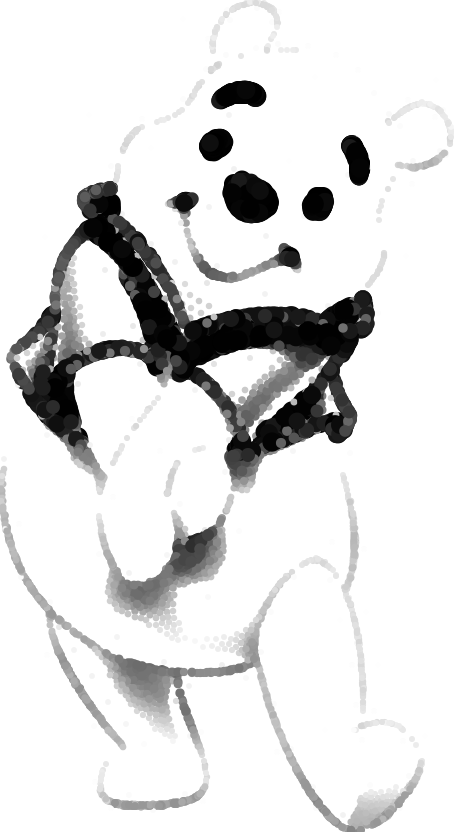
\includegraphics[width=.2\textwidth]{FIGS/pooh_grayscale/c1-h}
	\hspace{3mm}
	  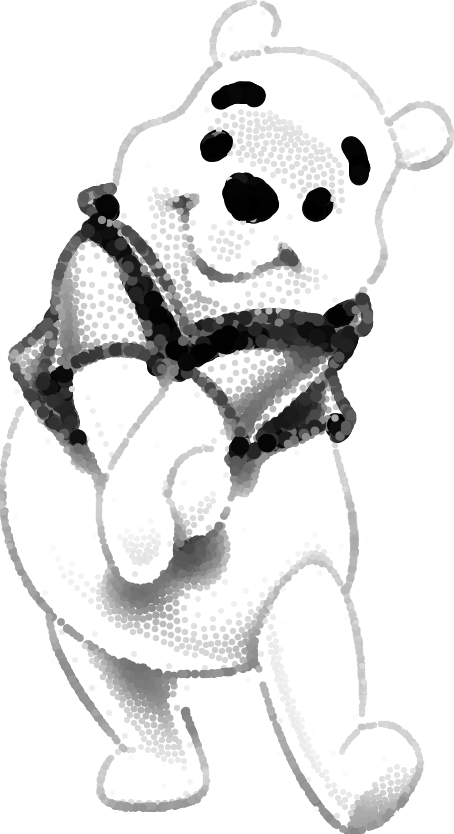
\includegraphics[width=.2\textwidth]{FIGS/pooh_grayscale/c2-h}
	\hspace{3mm}
	  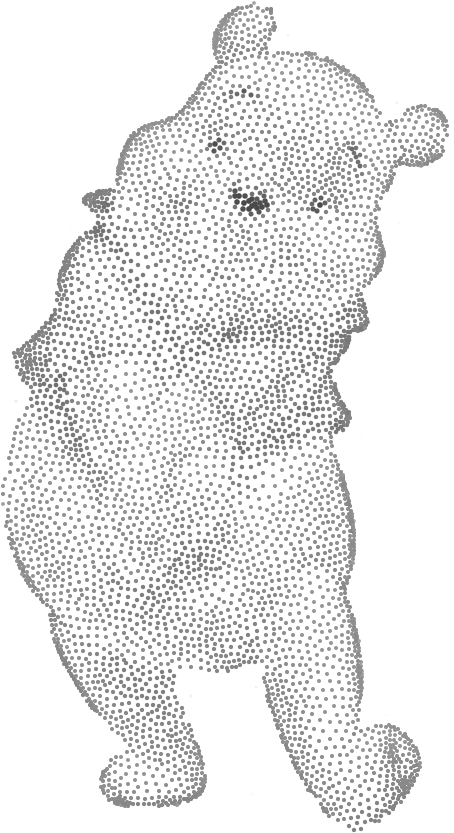
\includegraphics[width=.2\textwidth]{FIGS/pooh_grayscale/c3-h}
	\hspace{3mm}
	  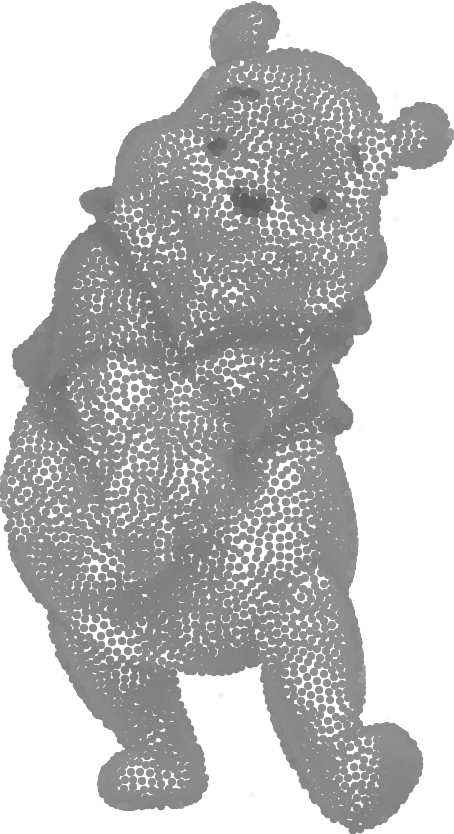
\includegraphics[width=.2\textwidth]{FIGS/pooh_grayscale/c4-h}
	  \caption{pooh as the contrast changes}
	  \label{fig:poohgrayscalechedcut}
	\end{figure}
	\begin{figure}[htbp]
	  \centering
	  \includegraphics[width=.2\textwidth]{FIGS/pooh_grayscale/c1-v}
	\hspace{3mm}
	  \includegraphics[width=.2\textwidth]{FIGS/pooh_grayscale/c2-v}
	\hspace{3mm}
	  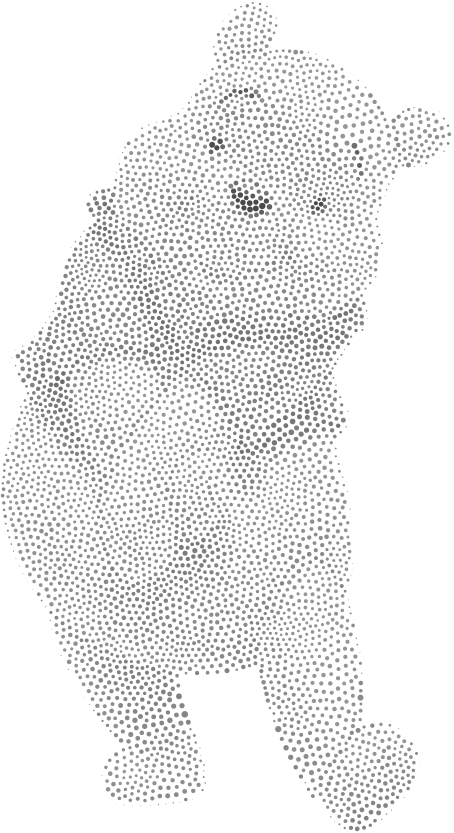
\includegraphics[width=.2\textwidth]{FIGS/pooh_grayscale/c3-v}
	\hspace{3mm}
	  \includegraphics[width=.2\textwidth]{FIGS/pooh_grayscale/c4-v}
	  \caption{pooh as the contrast changes}
	  \label{fig:poohgrayscalecvoronoi}
	\end{figure}
\subsection{Does the type of image (human vs. machine, natural vs. urban landscapes, photo vs.painting, etc) increase or decrease their difference?}%2.5
As I explained above, the results is affected by properties such as the number of stipples, the resolution, size or brightness. In addition, the number of iterations is important for the hedcuter method. These properties are independent on the type of image. They consist of two parts. One is the program option and the other is features of image not type. To be specific, image can have different size, brightness, contrast and color distribution. 
\begin{figure}[ht] 
	\begin{center} 
	\subfloat[Urban of Hedcuter]{
		\includegraphics[width=.4\textwidth]{FIGS/type/urban-10000-h}}
	\hspace{5mm}
	\subfloat[Urban of Voronoi]{
		\includegraphics[width=.4\textwidth]{FIGS/type/urban-v}}
	\caption{Urban} 
	\label{fig:urban}
	\end{center} 
\end{figure}
\begin{figure}[ht] 
	\begin{center} 
	\subfloat[Countryside of Hedcuter]{
		\includegraphics[width=.4\textwidth]{FIGS/type/countryside-10000-h}}
	\hspace{5mm}
	\subfloat[Countryside of Voronoi]{
		\includegraphics[width=.4\textwidth]{FIGS/type/countryside-v}}
	\caption{Country} 
	\label{fig:country}
	\end{center} 
\vspace{-2.0em}
\end{figure}
\clearpage
\begin{figure}[] 
	\begin{center} 
	\subfloat[Person of Hedcuter]{
		\includegraphics[width=.23\textwidth]{FIGS/type/person-10000-h}}
	\hspace{10mm}
	\subfloat[Person of Voronoi]{
		\includegraphics[width=.23\textwidth]{FIGS/type/person-v}}
	\caption{Person} 
	\label{fig:person}
	\end{center} 
\end{figure}
\begin{figure}[h] 
	\begin{center} 
	\subfloat[Robot of Hedcuter]{
		\includegraphics[width=.23\textwidth]{FIGS/type/bb8-10000-h}}
	\hspace{10mm}
	\subfloat[Robot of Voronoi]{
		\includegraphics[width=.23\textwidth]{FIGS/type/bb8-v}}
	\caption{Robot} 
	\label{fig:robot}
	\end{center} 
\end{figure}
\clearpage

\subsection{Are the outputs of these stippling methods different the hedcut images created by artists (e.g. those from the Wall Street Journal)?}
The images created by artists are good of quality since aritists can control unnatural clustering of stipples. However, as shown in the Figure \ref{fig:emmatompson}, the Voronoi method generates the high quality result enough to substitue the images by artists.
\begin{figure}[ht] 
	\begin{center} 
	\subfloat[Original image]{
		\includegraphics[width=.2\textwidth]{FIGS/wsj/emma-thompson-face}}
	\hspace{3mm}
	\subfloat[Hedcuter-15000]{
		\includegraphics[width=.2\textwidth]{FIGS/wsj/emma-thompson-face-15000-h}}
	\hspace{3mm}
	\subfloat[Voronoi-15000]{
		 \includegraphics[width=.2\textwidth]{FIGS/wsj/emma-thompson-face-15000-v}}
	\hspace{3mm}
	\subfloat[Wall Street Journal]{
		 \includegraphics[width=.19\textwidth]{FIGS/wsj/Emma-Thompson-wsj}}
	\caption{Emma Tompson} 
	\label{fig:emmatompson}
	\end{center} 
\end{figure}
\section{Improvement of hedcuter method}
\subsection{Adding functionality to generate colorful disks}
Orinally, the hedcuter generates grayscale results with non-black option. I edit the \textit{hedcut.cpp} to add functionality to generate colorful disks on the hedcuter program. To do this, I changed the part of reading a file to load the image in the BGR format. I used the grayscale image during the process of making initial points and computing weighted centroid voronoi tessellation using the \textit{cvtColor()}. Finally, I change the creating disks part. when I use a non-black option, it can calculate RGB from the RGB image.
	\begin{figure}[ht] 
	\begin{center} 
	\subfloat[5000 sample points]{
		\includegraphics[width=.25\textwidth]{FIGS/parrot/parrot-5000-h}}
	\hspace{5mm}
	\subfloat[10000 sample points]{
		 \includegraphics[width=.25\textwidth]{FIGS/parrot/parrot-10000-h}}
	\caption{Parrot of Hedcuter with non-black option} 
	\label{fig:parrotchedcuter}
	\end{center}
	\end{figure}
	\begin{figure}[ht] 
	\begin{center} 
	\subfloat[5000 stipples]{
		\includegraphics[width=.25\textwidth]{FIGS/parrot/parrot-5000-v}}
	\hspace{5mm}
	\subfloat[100000 stipples]{
	  \includegraphics[width=.25\textwidth]{FIGS/parrot/parrot-10000-v}}
	\caption{Parrot of Voronoi with colour option} 
	\label{fig:parrotcvoronoi}
	\end{center} 
	\end{figure}
\clearpage


\section{Results Analysis and Discussions}
My first challenge came from installing OpenCV and BOOST. I tried several times and downloaded lots of versions. To be specific, BOOST should be built with 32 address-model option. After setting, I experienced the second difficulty. The programs were really slow so that I had to wait too much time to run the programs. I could resolve this problem using release mode. Since I was totally unfamiliar with OpenCV, I referred to OpenCV documentation \href{http://docs.opencv.org/}{OpenCV docs}.  I struggled sometimes because I referred documentations of different versions. For example, \textit{scalar(a, b, c)} uses a BGR color in some version. Even though I could not finish the midterm perfectly, I could improve my skills to read the open source and use it. I studied two stippling methods. They generate good quality results in most cases. I calculated the elapsed time of each program to compare their performance. For comparison, the Voronoi method produces better result. However, if we run the Hedcuter with enough iterations and a appropriate disk size, it also generates high quality results. 
\bibliographystyle{plain}
\bibliography{report}

\end{document}


